\documentclass{article}
\usepackage{amsmath}
\usepackage{amssymb}
\usepackage{graphicx}
\usepackage{hyperref}
\usepackage[version=4]{mhchem}


\begin{document}
\section*{Problem}
(Phillips Academy Prize Exam) In right triangle \(A B C\), angle \(C\) is the right angle. \(P, Q\) and \(R\) are points which divide \(A B\) into four equal parts. \(S\) and \(T\) are the midpoint of \(B C\) and \(A C\), respectively. \(A B\) equals 24 inches. Find the perimeter of PRST.\\
\centering
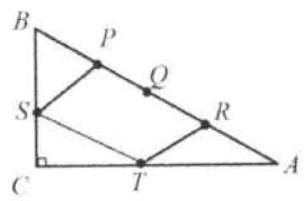
\includegraphics[width=\textwidth]{images/044(3).jpg}

\section*{Solution}
36.\\
Draw median \(C Q\). Since the median to the hypotenuse of a right triangle is half the hypotenuse,\\
\(C Q=\frac{1}{2} A B=\frac{24}{2}=12\).\\
Since \(S P, R T\), and \(S T\) are midlines,\\
\(S P=\frac{1}{2} C Q=\frac{12}{2}=6=R T\) and \(S T=\frac{1}{2} A B=\frac{24}{2}=12\).\\
\centering
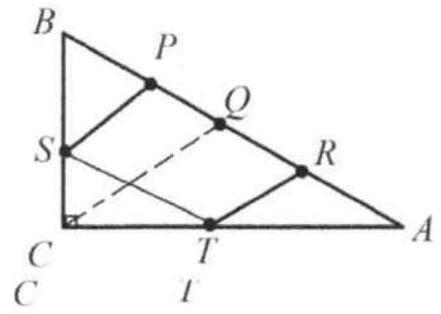
\includegraphics[width=\textwidth]{images/047(2).jpg}

The perimeter of PRST is 36 .

\end{document}
